\chapter{Introduction}

\section{Introduction to LaTeX}
LaTeX is a typesetting system that is widely used by the scientific community for document preparation and typesetting. It is especially useful for writing documents that include complex mathematical expressions and non-Latin scripts.


\section{Template Roadmap}

%---Guidelines---
\subsection*{Template Roadmap (do not include in final document)}
This LaTeX template is designed with a modular structure for easier management and customization. The template is broken down into separate files for each major section of your paper, all of which are combined into the final document using the main.tex file. Here's a breakdown of the file structure:

\begin{itemize}
    \item \textbf{main.tex}: This is the main file that you compile to create your document. It includes directives to incorporate all the other parts of your template.
    \item \textbf{chapters}: This directory contains separate .tex files for each chapter or major section of your document. These files are included into the final document by the main.tex file.
    \item \textbf{images}: This directory contains any image files that you want to include in your document.
    \item \textbf{includes}: This directory contains .tex files for smaller, often reusable sections of your document, like the abstract, dedication, and rights. It also contains the .bib file for your bibliography.
\end{itemize}

To set the Overleaf compiler to XeLaTeX, you can follow these steps:
\begin{enumerate}
    \item Click on the "Menu" button in the top left corner of the Overleaf editor.
    \item In the settings panel that opens, find the "Compiler" setting under the "Settings" section.
    \item Click on the dropdown menu and select "XeLaTeX".
    \item Click on "Done" to save your changes.
\end{enumerate}

Remember, the structure provided here is a guide and can be adapted to fit your specific needs.
%---End of Guidelines---

\section{Basic LaTeX Usage}
Here, we will explain some basic usage commands. Please note that these are very basic and can be easily learned in 30-60 minutes. If you are more of a visual learner, check out the following YouTube tutorial:
https://www.youtube.com/watch?v=zqQM66uAig0

\subsection{Sections and Subsections}
You can organize your document into sections and subsections using the \verb|\section{section name}| and \verb|\subsection{subsection name}| commands.

\subsection{Lists}
You can create bulleted and numbered lists in LaTeX.

Bulleted List:
\begin{itemize}
    \item Item 1
    \item Item 2
\end{itemize}

Numbered List:
\begin{enumerate}
    \item First Item
    \item Second Item
\end{enumerate}

\subsection{Images}
To add an image, you use the \verb|\includegraphics| command. Make sure to add the graphicx package in your preamble. Here is an example of its usage:

\begin{figure}[ht]
    \centering
    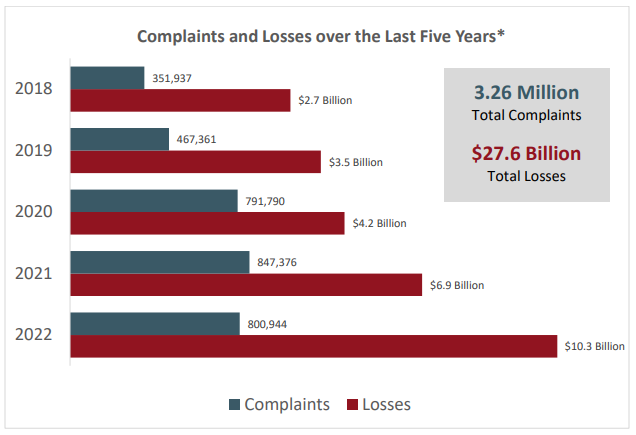
\includegraphics[width=350pt]{images/ic3_annual.png}
    \caption{FBI's 2022 Internet Crime Complaint Center (IC3) Annual Internet Crime Report}
    \label{fig:ice3_annual}
\end{figure}

\begin{verbatim}
\begin{figure}[h]
\centering
\includegraphics[width=0.5\textwidth]{image_file}
\caption{Caption of the image.}
\label{fig:my_label}
\end{figure}
\end{verbatim}

\subsection{Tables}
To add a table, you can use the table and tabular environments.

\begin{table}[ht]
\centering
\begin{tabular}{|c|c|}
\hline
Header 1 & Header 2 \\
\hline
Item 1   & Item 2   \\
\hline
\end{tabular}
\caption{Caption of the table.}
\label{tab:my_label}
\end{table}



\begin{verbatim}
\begin{table}[h]
\centering
\begin{tabular}{|c|c|}
\hline
Header 1 & Header 2 \\
\hline
Item 1   & Item 2   \\
\hline
\end{tabular}
\caption{Caption of the table.}
\label{tab:my_label}
\end{table}
\end{verbatim}

\subsection{Citing References}

References are an important part of any academic document. They not only acknowledge the work of others, but also allow readers to verify and follow-up your work. LaTeX makes citing references quite easy with the use of BibTeX, a tool for formatting lists of references.

BibTeX database files have a simple structure and they are easy to create. A `.bib` file is already included in this template in the `includes/` folder. An example of how to add a reference to this file is shown below:

\begin{verbatim}
@article{
    author = {John Doe},
    title = {Title of the Paper},
    year = {2020},
    journal = {Journal Name},
    volume = {4},
    pages = {10-20},
    publisher = {Publisher}
}
\end{verbatim}

Once your references are included in the `.bib` file, you can cite them in your text using the `\cite{}` command. The argument to the `\cite{}` command is the citation key, which is a unique identifier for each reference. In the example above, the citation key is `Doe2020`.

Here is an example of how to use the `\cite{}` command:

\begin{verbatim}
As stated by Doe \cite{Doe2020}, the usage of LaTeX simplifies document preparation.
\end{verbatim}

In the final document, this would appear as:

\begin{quote}
As stated by Doe [1], the usage of LaTeX simplifies document preparation.
\end{quote}


\subsection{Mathematical Expressions}
LaTeX is great for typesetting mathematical expressions. Enclose inline mathematical expressions with \$. For example, \verb|$E = mc^2$| will produce \(E = mc^2\). For numbered equations on their own lines, use the equation environment.

\begin{verbatim}
\begin{equation}
a^2 + b^2 = c^2
\label{eq:pythagorean}
\end{equation}
\end{verbatim}

\subsection{Page Breaks}
You can force a page break using the \verb|\clearpage| command. This is particularly useful when you want to control where new content starts.

\begin{verbatim}
\clearpage
\end{verbatim}

\subsection{Vertical Spacing}
You can control vertical spacing using the \verb|\vspace{length}| command. The length can be specified in various units, such as pt (points), mm (millimeters), cm (centimeters), in (inches), em (the width of the letter M in the current font), and ex (the height of the letter x in the current font).

\begin{verbatim}
\vspace{1cm}
This line is 1 cm below the previous line.
\end{verbatim}

\subsection{Horizontal Spacing}
For horizontal spacing, use the \verb|\hspace{length}| command. The length units are the same as for \verb|\vspace|.

\begin{verbatim}
This is \hspace{2cm} two cm space.
\end{verbatim}

\subsection{New Paragraphs and Line Breaks}
To start a new paragraph, leave a blank line in your LaTeX code. To force a line break without starting a new paragraph, use the \verb|\\| command.

\begin{verbatim}
This is a paragraph.

This is another paragraph.\\
This is a new line in the same paragraph.
\end{verbatim}

Remember that LaTeX is designed to provide excellent typography and layout out of the box, so manual spacing and page breaks should generally be used sparingly.
